\documentclass[aspectratio=169]{beamer}
\usetheme{Madrid}
\usefonttheme{structurebold}
\usefonttheme[onlymath]{serif}
%\usepackage[utf8]{vietnam}
\definecolor{BKTemplate}{rgb}{0.11765, 0.30588, 0.47451}
\usecolortheme[named=BKTemplate]{structure}
\setbeamercolor{title}{fg=BKTemplate,bg=} 
\setbeamertemplate{caption}[numbered]

\usepackage{graphicx}
\usepackage{amsmath}
\usepackage{tcolorbox}
\usepackage[export]{adjustbox}
\usepackage{caption}

\usepackage[utf8]{inputenc}
\usepackage[T1]{fontenc}    % use 8-bit T1 fonts
\usepackage{url}            % simple URL typesetting
\usepackage{booktabs}       % professional-quality tables
\usepackage{amsfonts}       % blackboard math symbols
\usepackage{nicefrac}       % compact symbols for 1/2, etc.
\usepackage[disable]{microtype}      % microtypography (disabled for bitmap fonts)
\usepackage{mathtools}
\usepackage{multicol}
\usepackage{comment}
\usepackage{forest}
\usepackage[linesnumbered, ruled]{algorithm2e}
\usepackage{algorithmic}
\usepackage{xcolor}
\usepackage{colortbl}
\usepackage{graphicx}
\usepackage{diagbox}
\usepackage{tikz}
\usepackage{subcaption}
% \captionsetup[subfigure]{labelsep=space}
\usepackage{amsmath}
\usepackage{dsfont}
\usepackage{stmaryrd}
\usepackage[style=authortitle,backend=bibtex]{biblatex}
\usetikzlibrary{positioning}

\addbibresource{thesiscite.bib}
\renewcommand{\footnotesize}{\tiny}
\newcommand{\mathbi}[1]{\boldsymbol{#1}}
\newtheorem{proposition}{Proposition}

%------------------------------------------------------------
%This block of code defines the information to appear in the
%Title page

\title[SEMINAR] %optional
{\vspace*{1cm}\\\textbf{AI CITY CHALLENGE 2026 TRACK 3}\\\textbf{Anomalous Events in Transportation}}

\subtitle{}
\institute[HCMUT] % (optional)
{
  Faculty of Computer Science and Engineering\\
  Ho Chi Minh City University of Technology\\
  Vietnam National University Ho Chi Minh City
}

\date[MAY 2026] 

%End of title page configuration block
%------------------------------------------------------------



%------------------------------------------------------------
%The next block of commands puts the table of contents at the 
%beginning of each section and highlights the current section:

\AtBeginSection[]
{
  \begin{frame}
    \frametitle{Table of Contents}
    \tableofcontents[currentsection]
  \end{frame}
}
%------------------------------------------------------------


\begin{document}

% The next statement creates the title page.
\setbeamertemplate{background canvas}{
	
\includegraphics[width=\paperwidth,height=\paperheight]{images/FrontBackground.pdf}
}
\begin{frame}[plain]
\titlepage
\end{frame}


% Set background for ll pages
\setbeamertemplate{background canvas}{
	
\includegraphics[width=\paperwidth,height=\paperheight]{images/Background.pdf}
}

%---------------------------------------------------------
%This block of code is for the table of contents after
%the title page
\begin{frame}
\frametitle{Table of Contents}
\tableofcontents
\end{frame}
\section{Objective}
\begin{frame}
\frametitle{Objective}
\begin{itemize}
    \item \textbf{Objective:} Build a unified video understanding model or system to detect, reason about, and explain anomalous events in transportation surveillance.
    \item \textbf{Key Requirements:} Perform diverse reasoning tasks ranging from simple event verification to open-ended causal analysis.
    \item \textbf{Core Mechanism:} Requires explicit chain-of-thought reasoning grounded in temporal and spatial evidence.
\end{itemize}
\end{frame}
\section{Tasks}
\begin{frame}{Task Taxonomy}
    \framesubtitle{10 Tasks Across 3 Main Groups}
    \begin{itemize}
        \item \textbf{Basic Group (QA \& Verification):}
        \begin{itemize}
            \item Event Verification (with and without explanation)
            \item Multiple-Choice QA (with and without explanation)
            \item Open-Ended QA
        \end{itemize}
        \item \textbf{Scene Group (Context):}
        \begin{itemize}
            \item Scene Description (Static)
            \item Video Summarization (Dynamic)
        \end{itemize}
        \item \textbf{Temporal Group (Analysis):}
        \begin{itemize}
            \item Temporal Localization (When the anomaly occurred)
            \item Causal Linkage (What caused the anomaly)
            \item Event Description (What happened in the interval)
        \end{itemize}
    \end{itemize}
\end{frame}
\section{Training Data}
\begin{frame}
\frametitle{Training Data}
\begin{itemize}
        \item \textbf{Volume:} 44,040 annotations across 3,670 CCTV transportation videos ($\sim$26.1 hours total).
        \item \textbf{Data Sources:} Aggregated from 8 public open-source datasets (e.g., VAD-R1, TAD, Accident-Bench, UCF Crime).
        \item \textbf{Auto-Labeling Pipeline:} 
        \begin{itemize}
            \item \textbf{Gemini 3.1 Pro:} Used for video captioning and structured event descriptions.
            \item \textbf{Gemma-4:} Used for multi-task Q\&A with chain-of-thought reasoning.
        \end{itemize}
        \item \textbf{Human Context:} 910 videos utilize existing NVIDIA human annotations (bounding boxes, timestamps) as supplementary context.
    \end{itemize}
\end{frame}

\begin{frame}
\frametitle{Training Data}
\begin{figure}
    \centering
    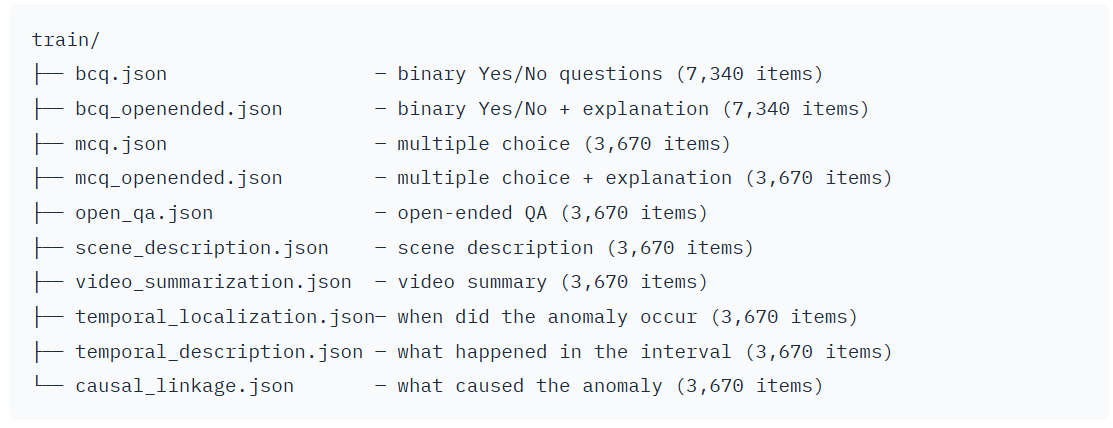
\includegraphics[width=0.9\textwidth]{images/train_structure.png}
\end{figure}
\end{frame}
\begin{frame}
\frametitle{Training Data}
\begin{figure}
    \centering
    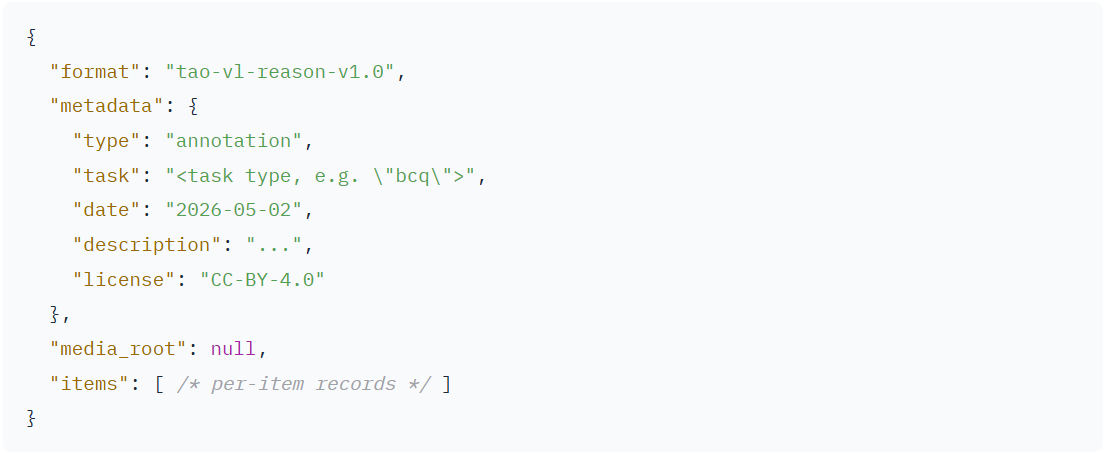
\includegraphics[width=0.9\textwidth]{images/json_structure.png}
\end{figure}
\end{frame}

\begin{frame}
\frametitle{Training Data}
\begin{figure}
    \centering
    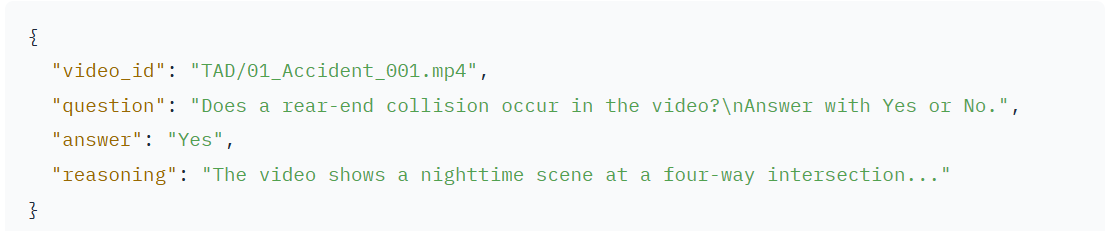
\includegraphics[width=0.9\textwidth]{images/item_structure.png}
\end{figure}
\end{frame}
\section{Test Data}
\begin{frame}{The Test Split}
    \begin{itemize}
        \item \textbf{Volume:} 960 human-curated annotations covering 80 short clips.
        \item \textbf{Source Material:} Clips are trimmed from 17 public YouTube videos, ensuring a distinct distribution from the training set.
        \item \textbf{Structure:} Retains the exact same 10 task types as the training data (spanning basic QA, scene understanding, and temporal reasoning).
        \item \textbf{Format:} Provided as a single combined file (\texttt{test.json}), but answers are redacted for the public leaderboard.
        \item \textbf{Data Access:} The \texttt{download\_test\_videos.py} script automatically uses \texttt{yt-dlp} and \texttt{ffmpeg} to fetch and trim the source clips.
    \end{itemize}
\end{frame}
\begin{frame}{The Test Split}
    \centering
    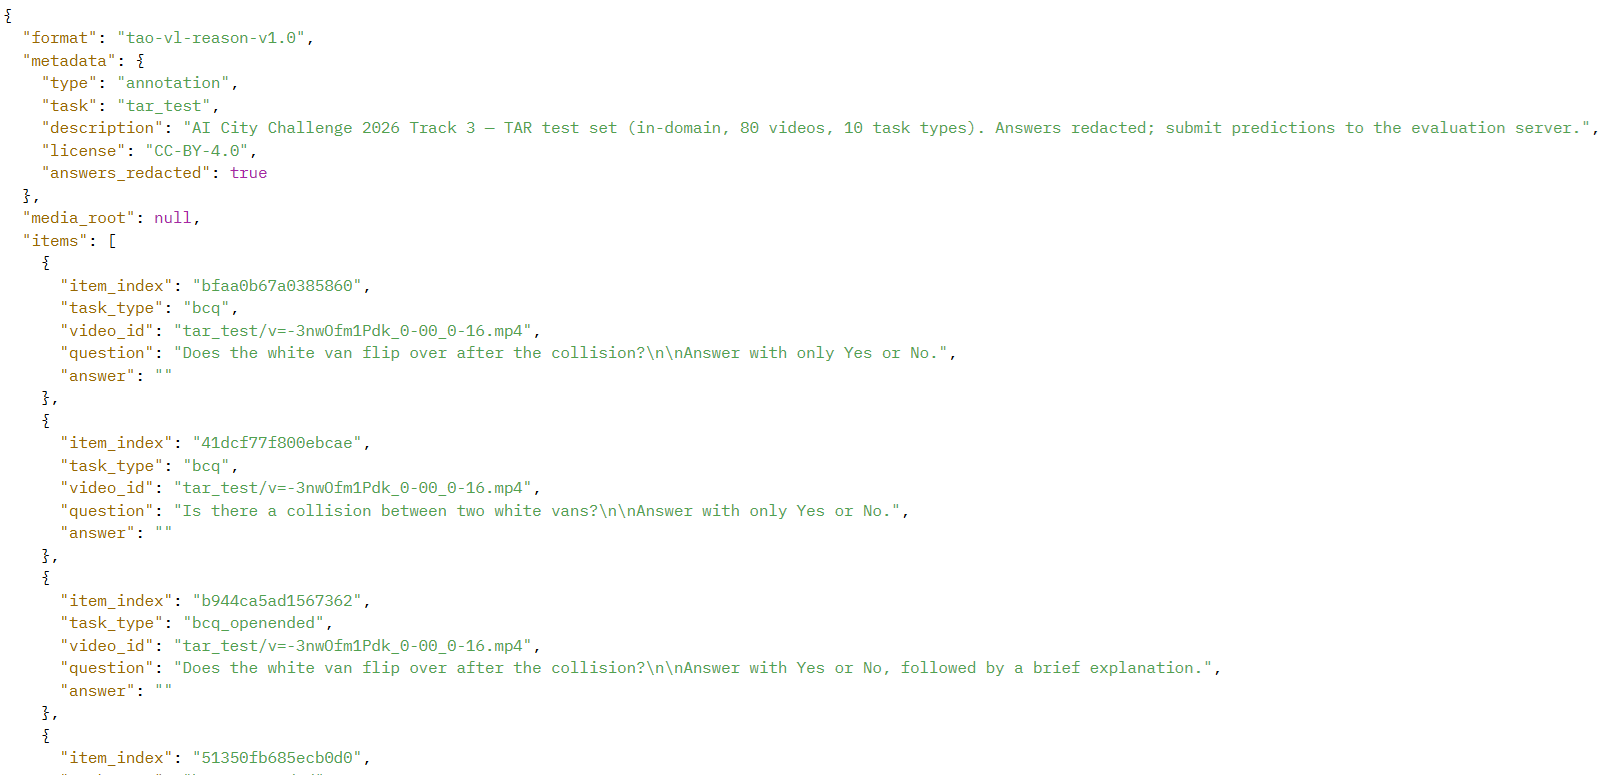
\includegraphics[width=\textwidth]{images/test_structure.png}
\end{frame}
\section{Submission Format}
\begin{frame}{Submission Format \& Local Validation}
    \begin{itemize}
        \item \textbf{Submission Format:} A single CSV file with exactly two columns:
        \begin{itemize}
            \item \texttt{item\_index}: The 16-hex sample ID from the test JSON.
            \item \texttt{prediction}: The model's raw output text (multi-line predictions allowed).
        \end{itemize}
        \item \textbf{Row Requirement:} Exactly 960 rows matching the test set IDs.
        \item \textbf{Local Validation:}
        \begin{itemize}
            \item The provided \texttt{evaluate.py} script runs in validation-only mode.
            \item It verifies CSV structure, completeness, and task-specific parseability (e.g., verifying Yes/No, single letter MCQ, or valid JSON for temporal boundaries).
        \end{itemize}
    \end{itemize}
\end{frame}
\section{Evaluation}
\begin{frame}{Evaluation \& Generalization}
    \framesubtitle{Rigorous Testing Methodology}
    \begin{itemize}
        \item \textbf{In-Domain Test Set:} Human-verified traffic anomaly videos, evaluated on the exact same 10 task types as the training set.
        \item \textbf{Out-of-Domain Set 1 (Fisheye):} Fisheye intersection traffic monitoring footage (tests generalization to a different task formulation).
        \item \textbf{Out-of-Domain Set 2 (Egocentric):} Dashcam video targeting pedestrian crossing intent prediction (tests generalization across visual domains and tasks).
    \end{itemize}
\end{frame}
\begin{frame}{Evaluation Metrics}
    \framesubtitle{Task-Specific Scoring}
    \begin{table}[]
        \centering
        \resizebox{\textwidth}{!}{%
        \begin{tabular}{ll}
            \toprule
            \textbf{Task Type} & \textbf{Metric} \\ \midrule
            Event Verification (\texttt{bcq}) & Yes/No accuracy (regex extraction) \\
            Multiple-Choice QA (\texttt{mcq}) & Letter accuracy (regex extraction) \\
            Temporal Localization & Mean IoU over \texttt{\{"start", "end"\}} JSON bounds \\
            Open-Ended / Explanatory Tasks & BERTScore F1 (\texttt{roberta-large}, rescaled) \\ \midrule
            \textbf{Overall Score} & \textbf{Unweighted mean of all per-task metrics} \\ \bottomrule
        \end{tabular}%
        }
    \end{table}
    \vspace{0.3cm}
    \textit{*Open-ended tasks include open QA, causal linkage, scene description, video summary, and QA with explanations.}
\end{frame}
\section{Approach}
\begin{frame}{Proposed Architecture: DINOv3-based Video-LLM}
    \framesubtitle{A Unified Perception-Reasoning Pipeline}
    
    \begin{columns}[T]
        \begin{column}{0.48\textwidth}
            \begin{block}{1. Spatial Perception (The Eyes)}
                \begin{itemize}
                    \item \textbf{Backbone:} DINOv3 (ViT-L/G).
                    \item \textbf{Strength:} Dense, self-supervised spatial features for zero-shot anomaly detection.
                    \item \textbf{Extract:} High-res patch embeddings per frame.
                \end{itemize}
            \end{block}
            
            \begin{block}{2. Temporal Bridge}
                \begin{itemize}
                    \item \textbf{Mechanism:} Perceiver Resampler or Temporal Transformer.
                    \item \textbf{Context:} Aggregates frame-level DINO features into spatio-temporal video tokens.
                \end{itemize}
            \end{block}
        \end{column}
        
        \begin{column}{0.48\textwidth}
            \begin{block}{3. Reasoning Engine (The Brain)}
                \begin{itemize}
                    \item \textbf{LLM Integration:} LLaVA-style projector maps tokens to LLM space (e.g., Llama 3 or Qwen2).
                    \item \textbf{CoT Output:} Fine-tuned to generate \textit{Reasoning} before \textit{Answer}.
                \end{itemize}
            \end{block}
            
            \begin{tcolorbox}[colback=blue!5,colframe=blue!75,title=Task-Specific Heads, fonttitle=\bfseries]
                \small
                \begin{itemize}
                    \item \textbf{Autoregressive:} QA, MCQ, Descriptions, and Causal analysis.
                    \item \textbf{Regression Head:} MLP-based 1D head for precise \textbf{Temporal Localization}.
                \end{itemize}
            \end{tcolorbox}
        \end{column}
    \end{columns}
\end{frame}
\end{document}